\documentclass{article}
\usepackage[margin=22mm]{geometry}
\usepackage{booktabs,graphicx}
\begin{document}
\title{MC connectivity with 100 micrometre simulation steps}\author{}\date{28 October 2026}\maketitle
Input: \texttt{events/0nubb\_100um.next.h5}, converted and verified using the
existing Julia hit-table converter. Compare the first 100 catalogue events of
this sample with the first 100 of the original double-beta sample. Samples are
compared as separate subsets; event IDs do not establish matching trajectories.
The 100 micrometre generation step is a user-provided simulation input.

KDT radius graphs use 0.5 mm voxels, source coordinates, all particles, and
Float32 calculations. No diffusion or fiducial selection is applied. All
connected components, including isolated nodes, are counted.
\begin{center}\begin{tabular}{rrrr}\toprule
Radius [mm] & Threshold [keV] & Original: single /100 & 100 $\mu$m: single /100\\\midrule
1.25 & 1 & 1 & 54 \\
1.25 & 0 & 1 & 55 \\
2 & 1 & 45 & 57 \\
\bottomrule\end{tabular}\end{center}

Primary hits are sorted separately by (MC time, hit ID). The two orderings agree
and there are no equal-time pairs in this subset. Distances are spatial chords
between stored deposits, not G4 path lengths. Voxel-transition statistics exclude
successive hits in the same cell and precede energy thresholding.
\begin{center}\begin{tabular}{lrrrr}\toprule
Positions & Pairs & Median [mm] & P99 [mm] & Maximum [mm]\\\midrule
Original hits & 191087 & 0.0994 & 0.1000 & 0.2000 \\
Voxel centres & 51386 & 0.5000 & 0.7071 & 0.8660 \\
\bottomrule\end{tabular}\end{center}
200 of 200 primary-electron voxel clouds form one connected
component at a radius of 1.25 mm with no energy threshold. Every measured
consecutive primary voxel transition lies within that radius. Thus the
step-induced primary fragmentation seen in the original sample is absent here.
Remaining event components require inspection of secondary deposits and
threshold effects; their count alone is not a background classification.

\noindent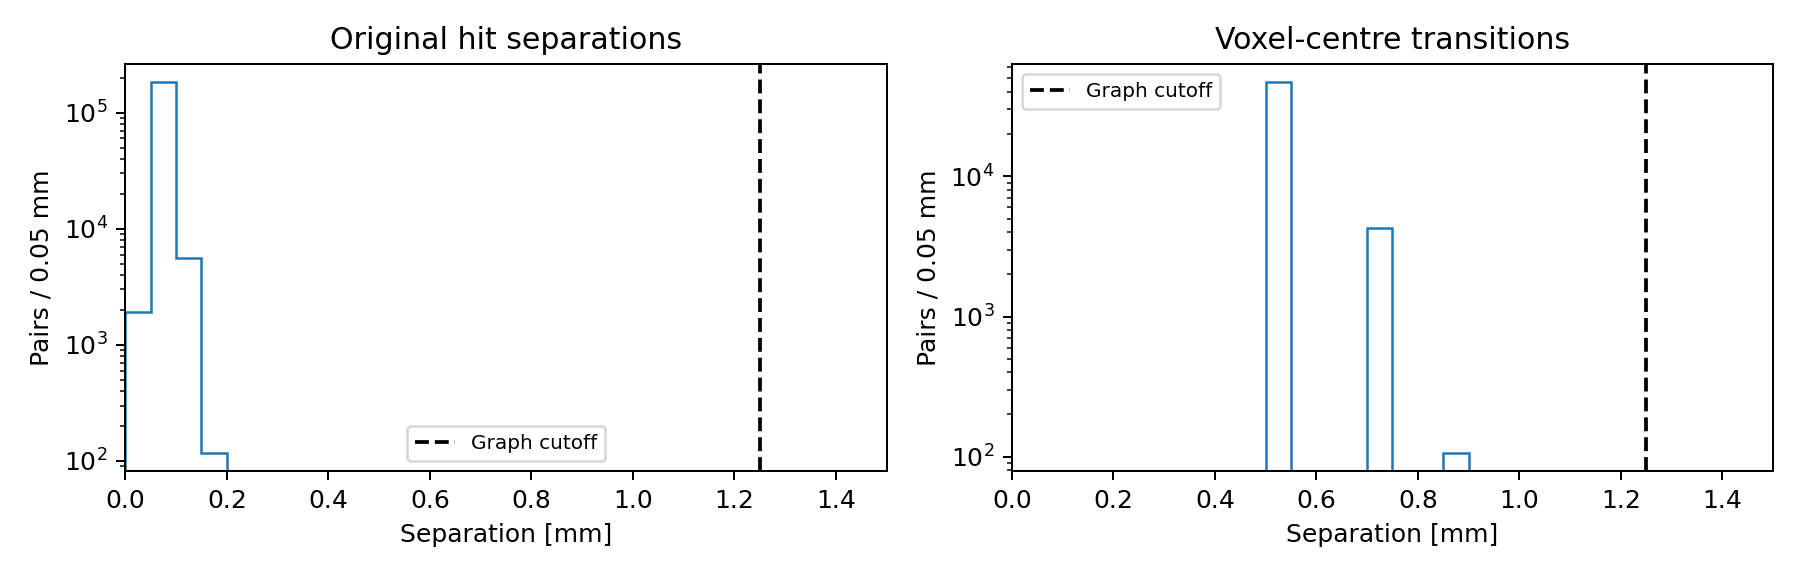
\includegraphics[width=\linewidth]{comparison_100um.png}

Numerical directory:\\ \texttt{results/event\_analysis/mc\_graph\_diagnostic/}\\
Files: \texttt{graph\_100um.h5}, \texttt{hit\_spacing\_100um.h5}, and \texttt{results.h5}.
\end{document}
